%!TEX root = ../thesis.tex
%*******************************************************************************
%****************************** Third Chapter **********************************
%*******************************************************************************
\chapter{Physics of Liquid Argon Time Projection Chamber}

% **************************** Define Graphics Path **************************
\ifpdf
    \graphicspath{{Chapter3/Figs/Raster/}{Chapter3/Figs/PDF/}{Chapter3/Figs/}}
\else
    \graphicspath{{Chapter3/Figs/Vector/}{Chapter3/Figs/}}
\fi

%********************************** %Opening  **************************************

The Liquid Argon Time Projection Chamber (LArTPC) stands as a high precision detector in neutrino physics.
The detector was first proposed in 1977 by Rubbia \cite{Rubbia}, bringing together the time projection chamber technology developed by Nygren \cite{Nygren1, Nygren2} and the liquid argon ionisation chamber developed by Willis and Radeka \cite{WillisRadeka}.
LArTPC provides an excellent spatial, calorimetry and timing resolution while enabling a high neutrino interaction rate.
This novel technology remains the primary choice for many neutrino experiments at Fermilab.

%overview
The following chapter will delve into principle operations of a LArTPC.
Sec. \ref{sec3:overview} provides an overview of the design of a LArTPC and the choice of liquid argon.
In Sec. \ref{sec3:creation}, a comprehensive discussion is presented on particle interactions with the liquid argon to produce ionisation electrons and scintillation photons, which are the observables of a LArTPC.
Following that, Sec. \ref{sec3:propagation} outlines the propagation of the resultant electrons and photons through the liquid argon medium.
Finally, Sec. \ref{sec3:detection} provides an insight into the detection mechanism of the ionisation electrons and scintillation photons using wire planes and novel optical detection technologies respectively.

\newpage

%********************************** %First Section  **************************************
\section{Overview of LArTPC}
\label{sec3:overview}
%1: Introduction
The Liquid Argon Time Projection Chamber (LArTPC) is the technology of choice for Fermilab's neutrino program, due to its ability to facilitate a high rate of neutrino interactions while maintaining an exceptional spatial, calorimetry, and timing resolution. 
Moreover, the abundant availability of argon is ideal for scaling detectors to a large target mass, reaching up to tens of kilotons of liquid argon.
Notably, the Short-Baseline Neutrino (SBN) programme \cite{SBNProgram} comprises of three LArTPC experiments of sizes in the hundreds of tons, located along the Booster Neutrino Beam (BNB): the Short-Baseline Near Detector (SBND) \cite{sbnd_det}, MicroBooNE \cite{ubooneDet}, and ICARUS \cite{icarus_det}.
This novel technology will also be utilised at the upcoming long baseline Deep Underground Neutrino Experiment (DUNE), of which its far detector is composed of four LArTPCs, boasting a total volume of 70 kilotons \cite{dunefd_det}.

%2: LArTPC description and figure 
A diagram illustrating the general operation principle of a LArTPC is provided in Fig. \ref{fig:LARTPC}.
Charged particles resulting from a neutrino interaction ionise argon atoms as they traverse through the detector medium, also producing scintillation photons in the process.
A high negative voltage is applied at the cathode plane, creating an electric field under which the ionisation electrons drift towards the anode.
\begin{figure}[htbp] 
\centering    
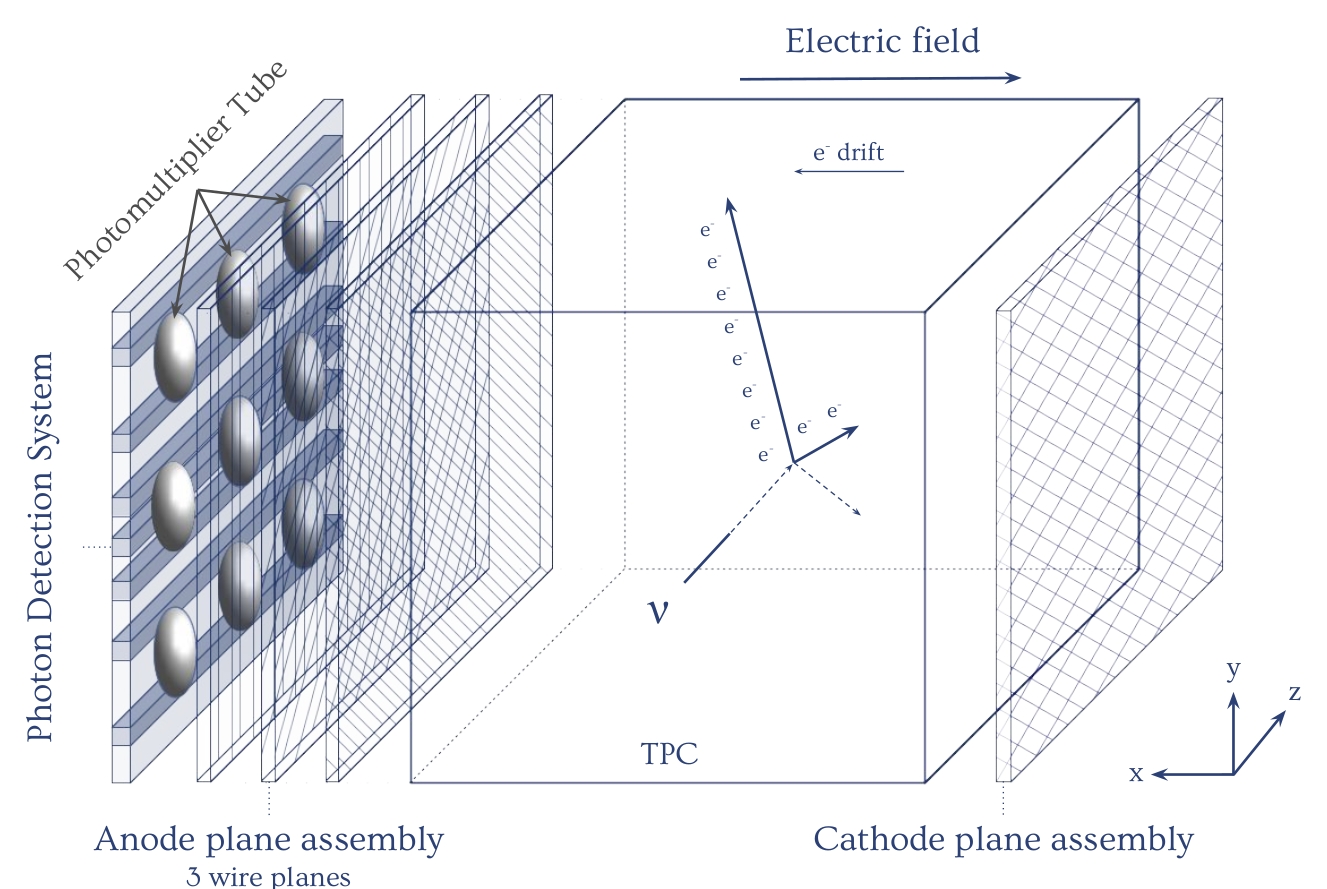
\includegraphics[width=0.65\textwidth]{LARTPC}
\caption[LARTPC]{
Illustration of a general LArTPC, depicting a cathode plane assembly on the edge of the TPC and an anode plane assembly in the opposite side along the x-direction.
Behind the wire planes at the anode is the PDS made up of 9 PMTs.   
An example neutrino interaction is shown, which produces two charged tracks (solid lines) and a neutral track (dashed line). 
The charged tracks produce ionisation electrons, which drift towards the anode in the opposite direction of the electric field. 
The neutral track does not ionise the argon atoms and thus is not directly visible in the detector. \cite{RhiannonPhD}.
}
\label{fig:LARTPC}
\end{figure}
Once arrive at the anode, the ionisation electrons induce signals on the inner wire planes and finally collected on the outermost plane.
The combination signals from these planes result in a high granularity three dimensional image of the interaction.
Since the wire planes are transparent to the scintillation photons, an additional Photon Detection System (PDS) is installed behind the wire planes, gaining additional calorimetry and precise timing information of the interaction.

%add why argon as target material
Specifically chosen for measuring neutrino cross sections, liquid argon has a high density of 1.39 gcm$^{-3}$ and a high atomic mass of 40.
The probability of neutrino interactions increases with the number of nucleons in the detector volume, and liquid argon, therefore, enables a high rate of neutrino interactions.
Furthermore, given that argon is a noble element, the energy deposited by particles traversing through the medium can only be used for ionising electrons and producing scintillation photons.
This maximises the efficiency of energy transfer into observable signals for detection.
Additionally, liquid argon has a very high electron mobility, allowing for ionisation electrons to quickly drift under an electric field.
Recent technology advancements in purifying argon has resulted in stable and ultra pure argon, which ensures that electrons can transverse the drift distance towards detection without being captured \cite{ubooneEtime}.
Consequently, liquid argon continues to stand out as an advantageous target material for neutrino experiments. 


\section{Particle Interactions in Liquid Argon}
\label{sec3:creation}

%Ionisation
\subsection{Ionisation Electrons}

%Energy loss profile
Charged particles traversing a medium, such as liquid argon, undergo energy loss via ionisation, producing electrons. 
The typical energy loss profile is illustrated in Fig. \ref{fig:BetheBloch}, specifically for a muon traversing in a copper medium; however, the underlying principle is applicable to liquid argon.
The plot depicts the stopping power, which is the energy loss per unit length divided by the density of the target medium, against the momentum of the traversing particle \cite{Passage}.
In the range of energy relevant in liquid argon, heavy particles such as muons, pions, and protons, experience energy loss as described by the Bethe-Bloch formalism.
On the other hand, for lighter and highly relativistic particles, such as > 100 MeV electrons in liquid argon, the primary mechanism for energy loss is through radiative effects.
An example depicting both of these event topologies is presented in Fig. \ref{fig:track_shower}.

\begin{figure}[htbp] 
\centering    
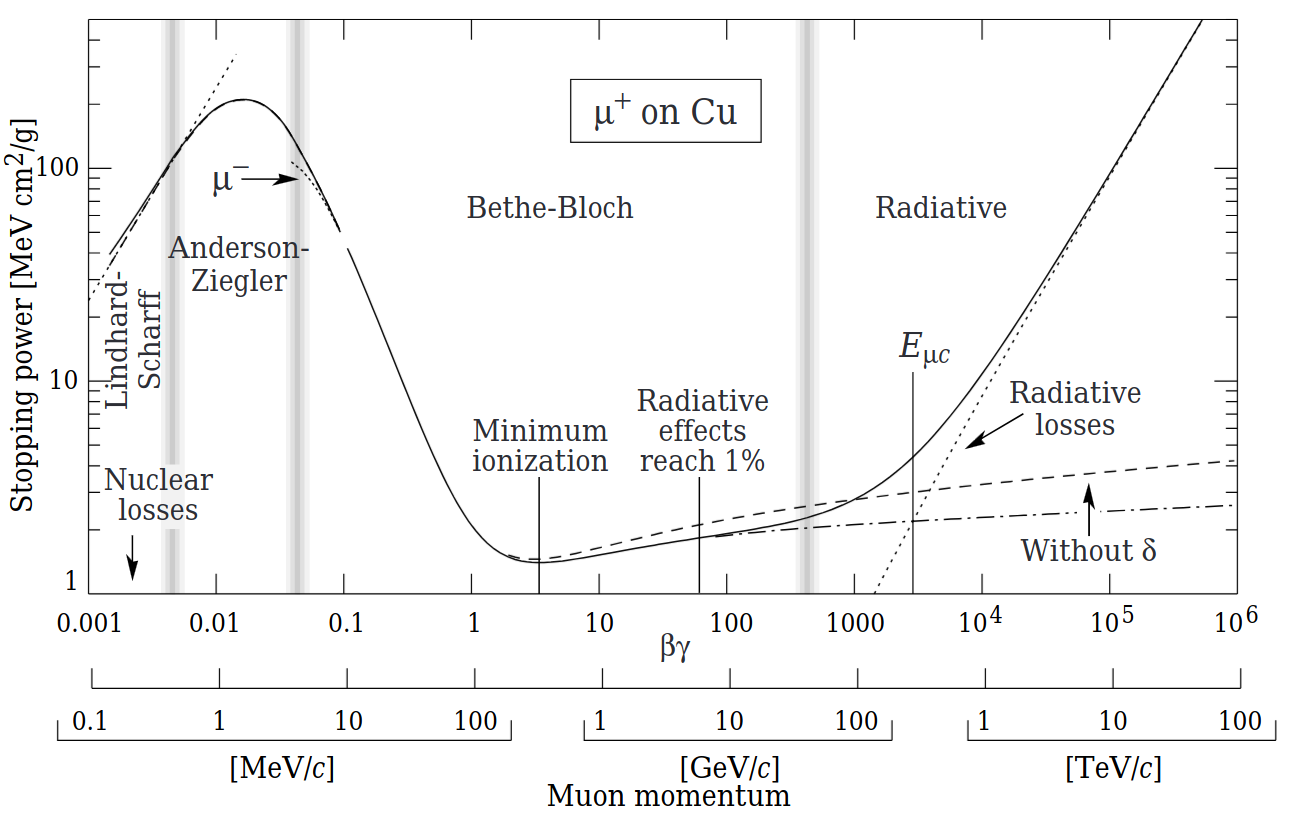
\includegraphics[width=0.85\textwidth]{BetheBloch}
\caption[BetheBloch]{
Example of particle energy loss in matter for a muon traversing a copper medium.
Energy loss for tracks is described by the Bethe-Bloch regime, followed by a rise in stopping power as the particle comes to a stop, representing the Bragg Peak.
Energy loss for showers is described by the radiative regime.
Fig. from \cite{Passage}.
}
\label{fig:BetheBloch}
%\end{figure}

%TODO: track and shower event display
\hfill
\break
%\begin{figure}[btp] 
\centering    
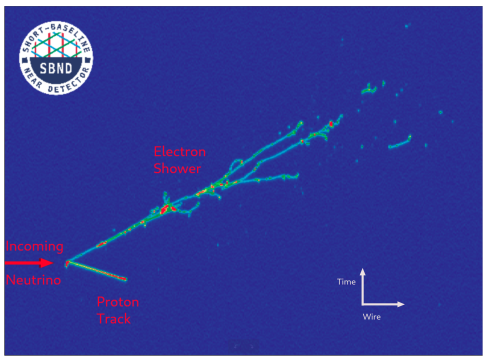
\includegraphics[width=0.6\textwidth]{temp}
\caption[track_shower]{
An event display of a charged current neutrino event, showing a track-like and a shower-like topology.
The track topology is from energy deposition of a proton, whereas the shower topology is from energy deposition of an electron interacting in liquid argon.
}
\label{fig:track_shower}
\end{figure}

%Track like
Muons, pions and protons interact electromagnetically with argon atoms as they propagate through liquid argon, primarily via Multiple Coulomb Scattering (MCS), freeing electrons along their trajectories.
These trajectories, typically following straightly lines, are referred to as \textit{tracks}.
As shown in Fig. \ref{fig:BetheBloch}, the MSC process is dependent on the momentum of the traversing particle.
Within the momentum range of 1 - 100 MeV, the energy deposited per unit length via ionisation, denoted as $dE/dx$, remains generally constant, often referred to as Minimum Ionising Particle (MIP).
In this MIP region, $dE/dx$ is described by a Landau-Gaussian Convolution. 
When the particle comes to a stop, the energy deposited arises, forming the so called Bragg peak.
The energy loss profile described here is dependent on the mass of the traversing particle, making it a valuable tool for Particle IDentification (PID) \cite{argoneut}.
This method is the most effective for protons separation from muons and pions, due to protons being significantly heavier.


%Shower like
Electrons with energy above the critical energy, which is the point at which losses due to ionisation are equal to losses from radiation, deposit energy via radiative effects \cite{uboone_gamma}.
The critical energy for electrons in liquid argon is 39 MeV.
This process typically results in cones of electromagnetic activities, commonly referred to as \textit{showers}. 
In the energy range relevant in a LArTPC, typically between 0.1 - 1 GeV, showers deposit energy over a distance of $\sim$1 m, and the shower length is logarithmic in energy.

Photons, being neutral particles, can travel some distance without ionising and before depositing energy inside the liquid argon \cite{uboone_gamma}.
This creates a gap between the interaction vertex and the start of the shower, known as the \textit{conversion gap}.
Photons can deposit energy via two interaction modes as illustrated in Fig. \ref{fig:uboone_gamma}.
At low energies, the primary process is Compton scattering, of which the radiation length is 14.1 cm.
However, at higher energies, pair production becomes the dominant effect, producing an $e^{+}e^{-}$ pair.
\begin{figure}[htp] 
\centering    
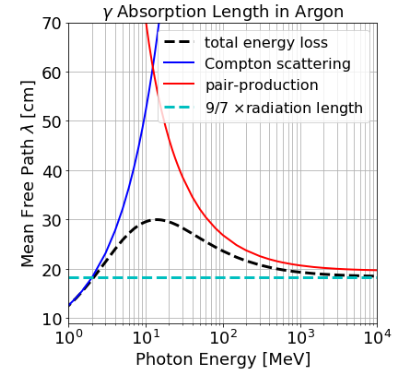
\includegraphics[width=0.40\textwidth]{uboone_gamma}
\caption[uboone_gamma]{
Plot showing the mean free path of photons traversing in liquid argon as a function of their energies.
In cyan is the conversion gap of 18.1 cm, which is 9/7 the radiation length.
Fig. from \cite{uboone_gamma}.
}
\label{fig:uboone_gamma}
\end{figure}
Both the energy loss profiles and the conversion gaps can be utilised to distinguish between electrons and photons. 


\subsection{Scintillation Photons}

%Scintillation light
Charged particles traversing liquid argon also produce scintillation photons, through two different processes, both resulting in an argon excimer ($Ar_{2}^{*}$) shown in Fig. \ref{fig:recomb_diagram}.
The first process is known as a self-trapped exciton.
This begins when the charged particle does not have sufficient energy for ionisation, and hence, it excites the argon atom upon collision instead.
The excited argon atom self-traps with another argon atom, forming an argon excimer .
The second process is known as recombination.
Ionisation in liquid argon produces a free electron and an argon ion ($Ar^{+}$).
The electron can either escape and drift towards the anode for detection, or recombine with an argon ion and an argon atom, forming an argon excimer.
The resulting argon excimer is short-lived and undergoes radiative decay into two ground-state argon atoms.
This process produces scintillation photons with a wavelength of 128 nm in the Vacuum UltraViolet (VUV) range \cite{Lariat}.

\begin{figure}[hbtp] 
\centering    
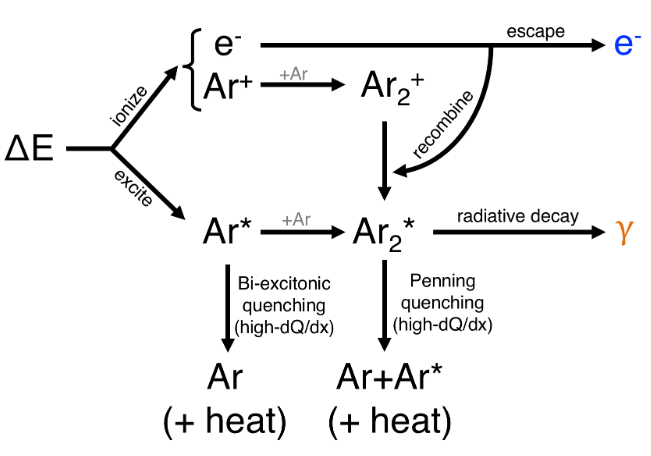
\includegraphics[width=0.6\textwidth]{recomb_diagram}
\caption[recomb_diagram]{
Diagram illustrating the production of ionisation electrons and scintillation photons from energy deposition processes in liquid argon.
Fig. from \cite{Lariat}.
}
\label{fig:recomb_diagram}
\end{figure}

The timing constant of the radiative decay depends on the excitation state.
The singlet state has a shorter mean lifetime with a decay constant $\tau_{1} \approx 6 - 7$ ns, while the triplet state has a longer mean lifetime with a decay constant $\tau_{3} \approx 1.5 - 1.6$ $\mu$s \cite{photon_lifetime}.
These are referred to as the fast (or prompt) and slow (or late) components, respectively. 
The time-dependent probability of light emission in pure liquid argon can therefore be modelled as
\begin{equation}
	l(t)=\frac{A_{1}}{\tau_{1}}\exp{\left(-\frac{t}{\tau_{1}}\right)} +\frac{A_{3}}{\tau_{3}}\exp{\left(-\frac{t}{\tau_{3}}\right)}
\end{equation}
where $A_{1}$ and $A_{3}$ are the decay amplitudes of the singlet and triplet state. 

%TODO: Add time distribution graph, see Patricks

%Quenching
Liquid argon serves as an excellent medium for producing scintillation photons, such that the light yield is as high as $\sim$40,000 photons per MeV of deposited energy in the absence of an electric field \cite{light_yield}.
In a typical electric field at 500 V/cm, as configured in SBND, the light yield decreases to $\sim$20,000 photons per MeV of deposited energy, due to free electrons being drifted before recombination can occur \cite{light_yield_Efield}.
Furthermore, high ionisation density may lead non-radiative quenching effects \cite{Lariat}.
Contaminants in liquid argon, such as oxygen and nitrogen, can absorb energy from argon excitons and excimers, without emitting any photons.
 
\subsection{Recombination}
\label{sec:recomb}
%Recombination

The electron-ion recombination, as depicted in Fig. \ref{fig:recomb_diagram}, occurs almost immediately within 1-2 ns following the ionisation process.
The electron recombination survival probability, also known as \textit{recombination factor} $R$, is defined as following 
\begin{equation}
	R=W_{ion} \cdot \frac{dE/dx}{dQ/dx}
\end{equation}
where $W_{ion} = 23.6$ eV is the energy required to ionise an argon \cite{ion_e} and $dQ/dx$ and $dE/dx$ is the charge and energy loss per unit length respectively. 
In Fig. \ref{fig:recomb_graph}, a comparison of various recombination models with a non-linear dependence on $dE/dx$ is presented.
The Birks model has been disfavoured due to spurious values at high charge density \cite{argoneut_recomb}.
The Box model is based on columnar theory around the charge deposition, and its modified version with experimentally-derived parameters measured by the Argoneut experiment, has improved agreement with data at low charge density.
The modification accounts for the presence of an electric field and local ionisation density.
\begin{figure}[thp] 
\centering    
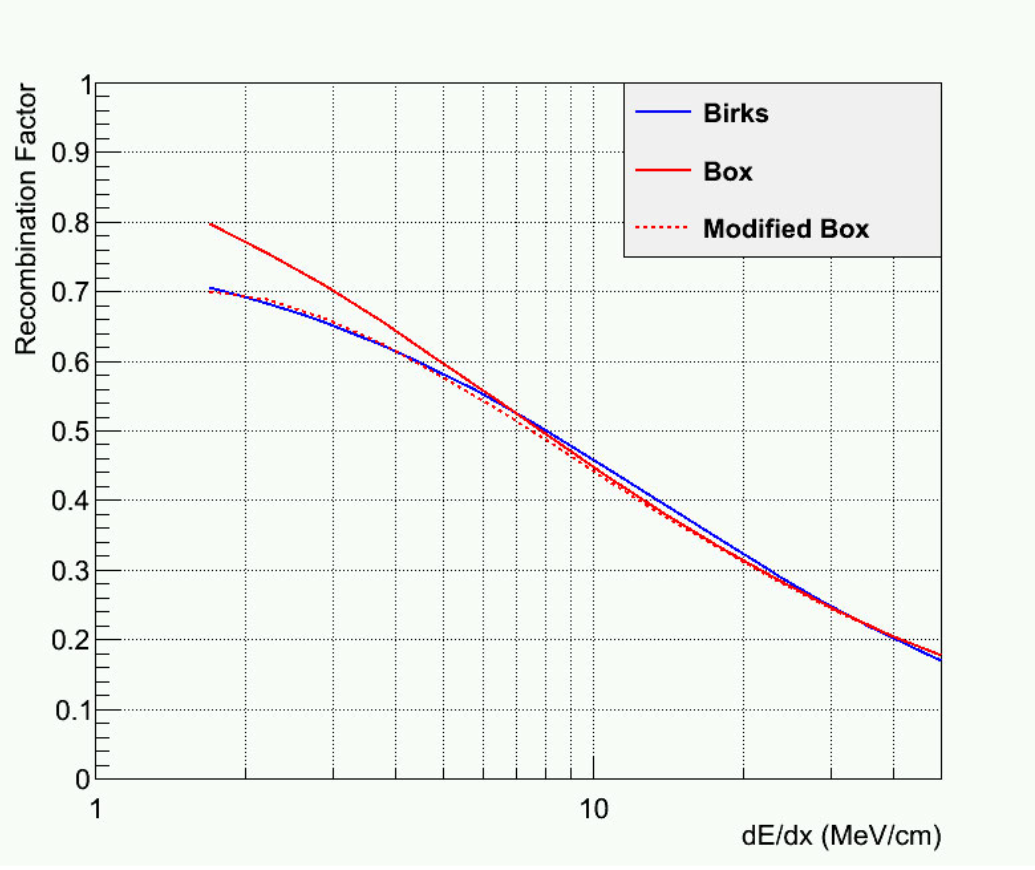
\includegraphics[width=0.6\textwidth]{recomb_graph}
\caption[recomb_graph]{
Graph showing recombination factor as a function of deposited energy density at an electric field of 500 V/cm. 
Fig. from \cite{argoneut_recomb}.
}
\label{fig:recomb_graph}
%\end{figure}
%\begin{figure}[tp] 
\hfill
\break
\break
\centering    
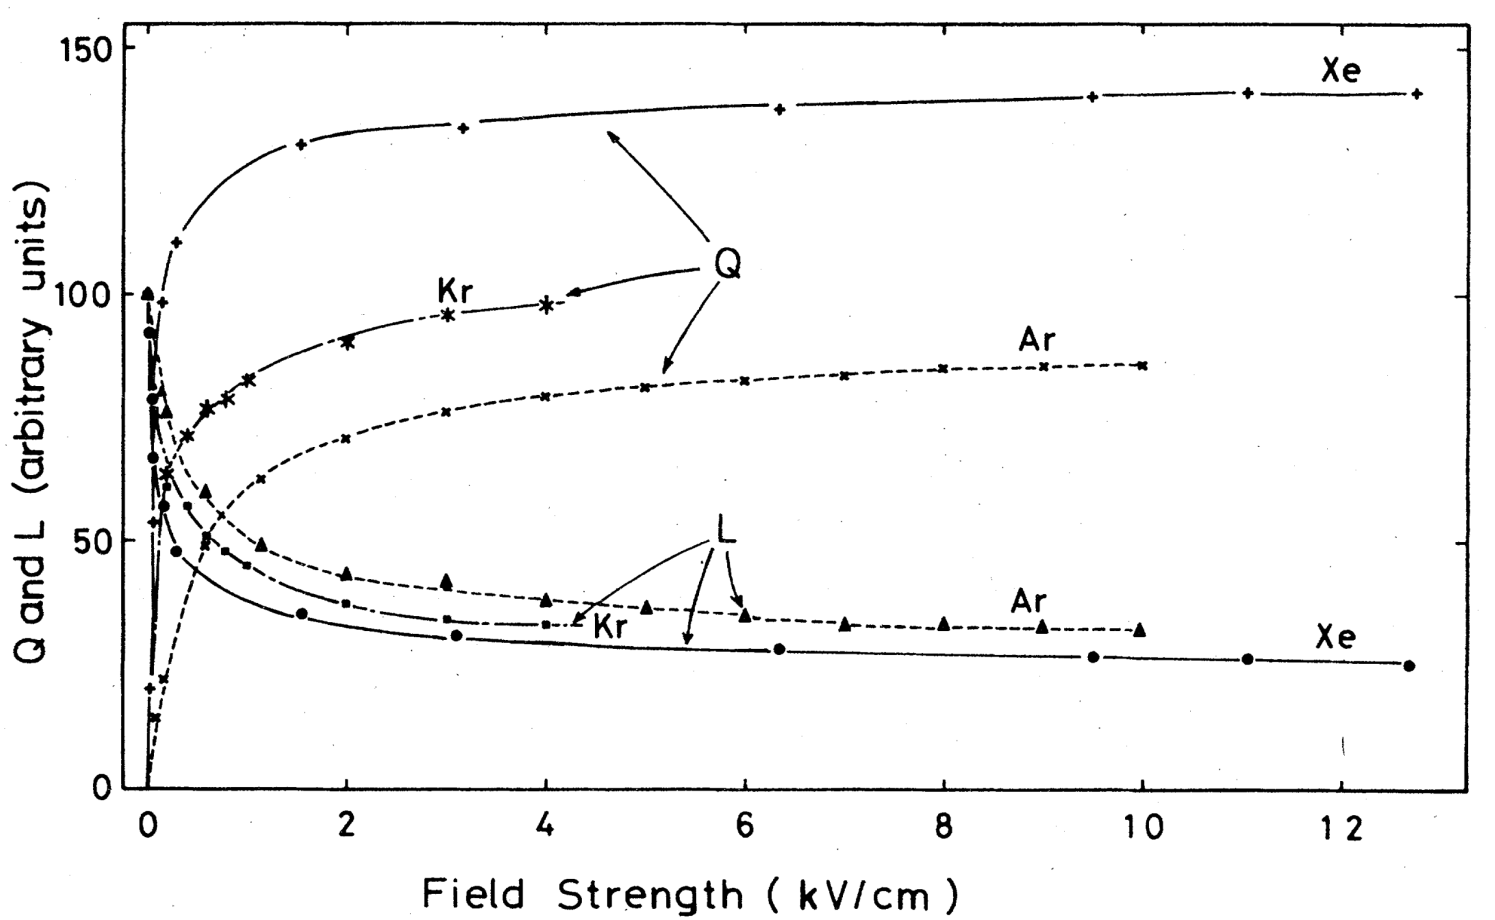
\includegraphics[width=0.7\textwidth]{QLAnti}
\caption[QLAnti]{
Charge ($Q$) and light ($L$) anti-correlation for noble elements like argon, xenon and krypton as a function of the electric field strength.
Fig. from \cite{QLAnti}.
}
\label{fig:QLAnti}
\end{figure}

%A popular model to describe this effect is the Box Model, based on columnar theory around the charge deposition \cite{box_model}. 
%The inverse Box Model equation is formulated as \cite{argoneut_recomb}
%\begin{equation}
%	\frac{dE}{dx} = \frac{1}{\beta}\left[ \exp{\left( \beta W_{ion}  \frac{dQ}{dx}\right)} -\alpha \right]
%\end{equation}
%where $\alpha$ and $\beta$ are experimentally derived parameters.
%Recombination is highly dependent on the electric field and the local charge density, which is folded into the $\beta$ parameter.
%ArgoNeuT experiment recently conducted a data-driven study on recombination in LArTPC, resulting in the ``Modified Box Model" with parameter $\alpha = 0.93$ and $\beta = 0.30 $ MeV/cm \cite{argoneut_recomb}.
%If not taken into account, the recombination can result in underestimating energy loss due to ionisation.

The dependence of recombination on the electric field leads to an anti-correlation between the charge and light yield $Q$ and $L$ respectively, such that \cite{argoneut_recomb}
\begin{gather}
	Q = N_{i}R \\ 
	L = N_{ex} + N_{i}(1 - R)
\end{gather}
where $N_{i}$ is the number of electron-ion pairs and $N_{ex}$ is the number of argon excitons.
A stronger electric field results in a higher number of ionization electrons being separated from the argon ions and drifted towards the anode for detection before recombination can occur. 
Conversely, scintillation photons are produced in the recombination process.
In the presence of an electric field, recombination decreases, leading to a reduction in light yield.
Furthermore, the recombination factor can be influenced at a local scale due to ionization density resulting from interacting particles.
Fig. \ref{fig:QLAnti} illustrates the anti-correlation between charge and light yield as a function of electric field strength for various noble elements.
The SBND detector operates with an electric field of 500 V/cm, a region where the energy deposition to ionization electrons and scintillation electrons are approximately equal \cite{QLAnti}.

%TODO: Check Gray's paper on recombination dependence of track angular
\section{Particle Propagation in Liquid Argon}
\label{sec3:propagation}

%Transportation of ionised electrons, diffusions, impurities
\subsection{Electrons Drift}
\label{sec:edrift}
\subsubsection{Diffusion}

%Electron drift under electric field
Ionised electrons that do not recombine drift towards the anodes under the effect of an electric field.
In a typical LArTPC with an electric field of 500 V/cm and a temperature of 87 K, the drift velocity of electrons is approximately 0.16 cm/$\mu$s \cite{drift_vel}.
As the electrons drift, they undergo diffusion, causing perturbations in their trajectories due to various effects, such as inelastic collisions.
Diffusion causes the shape of a cloud of electrons produced in a point like energy deposition to grow in volume while drifting.
The effects increase with respect to the drift distance, smearing both spatial and temporal resolutions.
The observed Gaussian profile $\sigma$ resulting from the response function of a charge deposition on the wire can therefore be modelled as \cite{uboone_diff} 
\begin{equation}
	\sigma^{2} (t) = \sigma^{2}_{0} + \left(\frac{2D}{v^{2}_{d}}\right)t
\end{equation}
where $\sigma_{0}$ is the initial profile without diffusion, $v_{d}$ is the drift velocity, $t$ is the drift time and $D$ is the diffusion coefficient.

Diffusion is parameterised in both the longitudinal direction $D_{L}$ and the transverse direction $D_{T}$, which are parallel and perpendicular to the drift direction respectively.
Longitudinal diffusion affects the temporal resolution, as individual electrons arrive at the wire either earlier and later relative to the electron cloud moving at the average drift velocity.
Transverse diffusion broadens the cross section of the electron cloud arriving at the original wire, causing electrons migrating to neighbouring wires.
Under the same conditions as the SBND detector, the diffusion coefficients have been measured to be $D_{L} = 7.2 $ cm$^{2}$/s and $D_T = 12.0 $ cm$^{2}$/s \cite{drift_vel}.

%TODO: Add how SBND measure diffusion (?)

\subsubsection{Attenuation}
%impurity: electron lifetime
Drifting electrons can be captured by electronegative impurities present in the liquid argon, most commonly oxygen and water \cite{protodune}.
This results in the attenuation of the electrons arriving at the wire, proportional to the drift distance. 
The amplitude of the electrons collected on the wire $Q_{wire}$ is typically modelled as an exponential suppression
\begin{equation}
	Q_{Wire} (t) = Q_{Dep} \cdot \exp\left(\frac{-t}{\tau}\right)
\label{eq:etime}
\end{equation}
where $Q_{Dep}$ is the original deposited charge, $t$ is the drift time and $\tau$ is the electron lifetime characterising the level of charge attenuation.
A high electron lifetime, resulting from a low level of contamination, is a critical operational factor for achieving high efficiency in energy reconstruction.
Recently reported from ProtoDUNE, which utilised the same membrane cryostat technology as SBND, the experiment measured a lifetime of $\sim$10 ms, equivalent to an oxygen purity of 3.4 ppt \cite{protodune}.
This lifetime is significantly larger than the drift time of SBND (1.25 ms), making this effect almost negligible. 

%TODO: Add how SBND measures electron lifetime and purification system (?)

\subsubsection{Space Charge Effect}
%space charge effect
Argon ions, produced as part of the ionisation process, drift towards the cathode at a slower velocity, more than five orders of magnitude slower than the electron drift velocity \cite{icarus_sce}.
Since SBND is a surface detector without an overburden, high exposure to cosmics rays leads to a high rate of ionisation.
The accumulation of slow-moving argon ions distorts the uniformity of the electric field, affecting both its intensity and direction.
This consequently impacts the charge deposition both spatially and calorimetrically.
This effect is referred to as Space Charge Effect (SCE).
The calorimetry effect arises due to the dependence of the recombination factor on the local distortion of the electric field.
The spatial effect is due to the deformation of tracks drifting in the distorted electric field as shown in Fig. \ref{fig:SCE}.
SCE impacts the track trajectories two-folds: causing bending away towards the detector edges and creating a bowed appearance towards the cathode.
\begin{figure}[htbp] 
\centering    
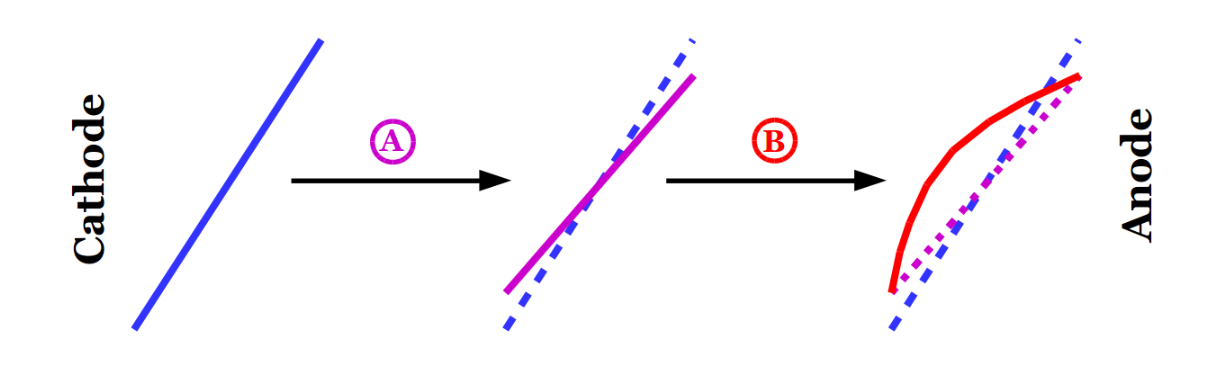
\includegraphics[width=0.8\textwidth]{SCE}
\caption[SCE]{
SCE impacts the track trajectories in two ways: causing bending away towards the detector edges, as indicated in the rotation A, and bowing towards the cathode, as indicated by transformation B.
Fig. from \cite{SCE}.
}
\label{fig:SCE}
\end{figure}
%TODO: something sounds fudgy
%Therefore, SCE worsens the spatial as well as energy resolution of a track reconstruction and consequently, particle identification.
%SBND will implement a dedicated laser calibration system \cite{}, as well as calibration using cosmics track crossing cathode and anode \cite{} to model the distorted electric field.
%Once measured, correction will be applied in the reconstruction. 

\subsection{Photons Propagation}

\subsubsection{Rayleigh Scattering}

%TODO: Check length, add group velocity/ rayleigh wavelength from Patrick's
Liquid argon is transparent to its own scintillation light, allowing emitted photons to propagate over long distances. 
As scintillation photons travel, they undergo various physical processes, including Rayleigh scattering, reflections and refractions at the boundaries of the detector material.
Rayleigh scattering, a first-order effect, involves photons elastically scattering off nuclei, altering their trajectories. 
Reflection off solid surfaces in the detector is a second-order effect. 
While these effects do not change the number of photons, they modify the paths of propagation and lengthen the travel time. 
The impact of these effects on the probability of photons reaching the PDS depends on the locations where the photons are created and their paths taken to arrive at the PDS. 
This consequently leads to a non-trivial distribution of photon arrival time at the PDS, and the travel time can range from a few to several tens of nanoseconds.
Particularly, this effect is the most impactful on the prompt component of scintillation photons.
%, which is crucial for the purpose of triggering (See Chapter \ref{}) and high-precision timing analysis (see Chapter \ref{}).
The Rayleigh scattering length $\lambda_{RS}$ for VUV photons in liquid argon has been reported to be around 50 cm \cite{rayleigh50} up to 110 cm \cite{rayleigh110}, which is comparable to the size of SBND.


\subsubsection{Absorption}
Scintillation photons can be absorbed by contaminants with a high cross-section for VUV photons, such as nitrogen \cite{photon_nitrogen} and methane \cite{photon_methane}. 
Other elements, like oxygen and water, have also been observed in commercial argon \cite{photon_commercial}. 
The total absorption of scintillation photons can be modelled as an exponential suppression of the number of photons as a function of the propagation distance, with the absorption length as a parameter (similar to Eq. \ref{eq:etime}).
The absorption rate is dependent on the Rayleigh scattering length. 
Photons with a shorter $\lambda_{RS}$ undergo longer and more indirect paths, increasing their probability of absorption before reaching the PDS.

\subsubsection{Wavelength Shifting}
\label{sec:wls}

%Scintillation photons in the VUV range are typically absorbed by detector materials without being detected. 
An enhancement method for scintillation light signals in LArTPC is wavelength shifting.
Specifically at SBND, TetraPhenyl Butadiene (TPB) is employed to shift the wavelenght of VUV photon from 128 nm to 430 nm, which falls within the visible light range.
TPB is utilised at two locations: first, it is evaporated onto the highly reflective foils located at the cathode, and second, it is coated on the optical windows of the photon detectors. 
In the former method, VUV photons arriving at the reflective foils are wavelength-shifted and reflected back towards the anode for detection.
In the latter method,  VUV photons arriving at the photon detectors are wavelength-shifted into the detectable wavelength range of the detectors.

The propagation characteristics of photons differ between the VUV and visible range.
As shown in Fig. \ref{fig:vuv_visible}, the high refractive index of liquid argon at 128 nm wavelength, approximately 1.38 \cite{lar_index}, results in a group velocity for VUV photons about twice slower than visible photons.
Moreover, the Rayleigh scattering length for VUV photons is two orders of magnitude smaller compared to visible photons.
Therefore, VUV photons are more susceptible to Rayleigh scattering and have a higher probability of absorption \cite{PatrickPhD}.
\begin{figure}[htp] 
\centering    
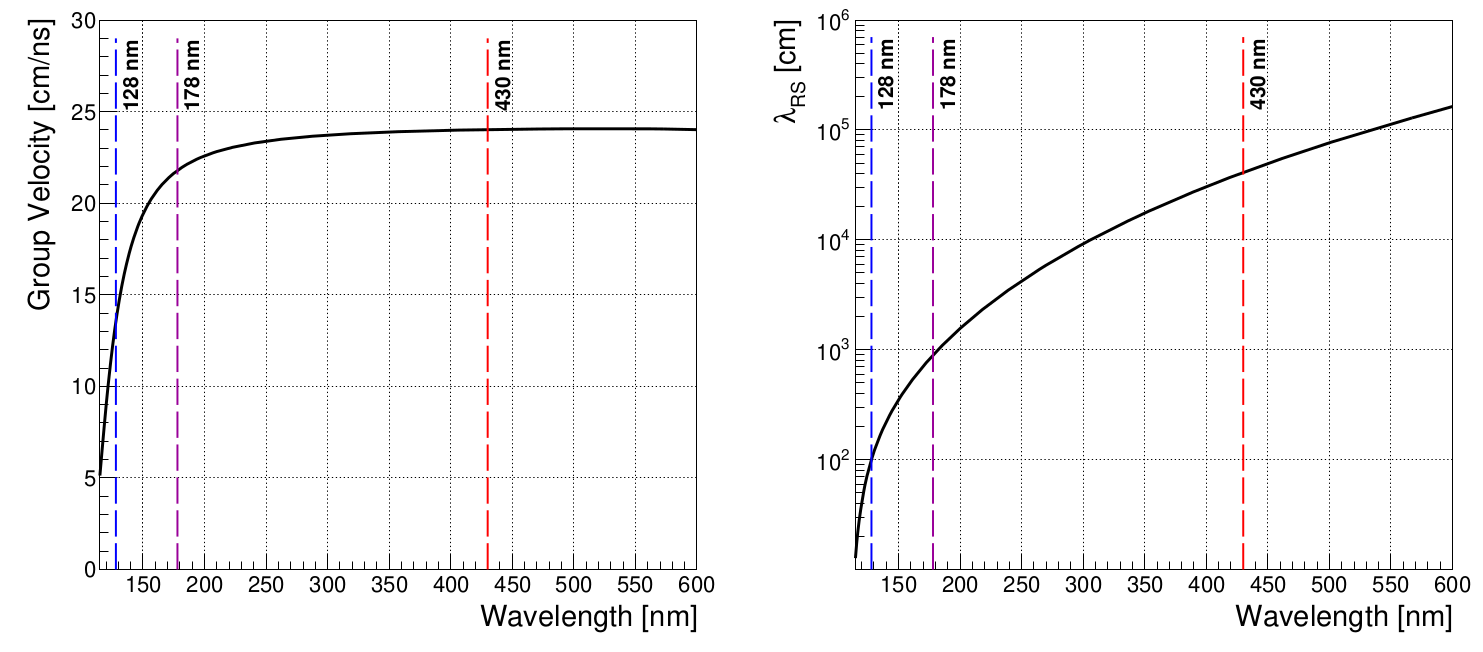
\includegraphics[width=0.85\textwidth]{vuv_visible}
\caption[vuv_visible]{
Graphs showing group velocity (left) and Rayleigh scattering (right) as a function of the wavelength of photons in liquid argon.
The lines at 128 nm, 178 nm and 430 nm are the wavelengths of scintillation photons in liquid argon, xenon-doped argon and from re-emission by wavelength-shifting by TPB. 
Fig. from \cite{PatrickPhD}.
}
\label{fig:vuv_visible}
\end{figure}
Conversely, visible photons that are reflected undergo longer propagation paths, Rayleigh scattering and propagating towards the cathode, wavelength-shifting and reflecting back the full width of the detector before reaching the photon detectors.
The spatial distribution of visible photons is more diffused and spread across a larger number of photon detectors compared to direct VUV photons \cite{PatrickPhD}.

Consequently, this leads to different arrival time and detection probability distributions for direct VUV and reflected visible photons.
The comparison of their light yield is shown in Fig. \ref{fig:light_yield_Diego} for TPB-coated and uncoated PMTs.
Closer to the anode, the light yield primarily comes from the direct VUV photons, detectable by coated PMTs.
Meanwhile, closer to the anode, and hence the reflective foils, the contribution to the light yield from reflected visible photons increased, which is detectable by both coated and uncoated PMTs.
ns.
The combined light yield from both components results in an improved overall light yield and a more uniform distribution across the drift length of the detector \cite{light_yield_Diego}.

\begin{figure}[htbp]
%TODO: Fix reference from Diego's talk to SBND PDS paper
\centering    
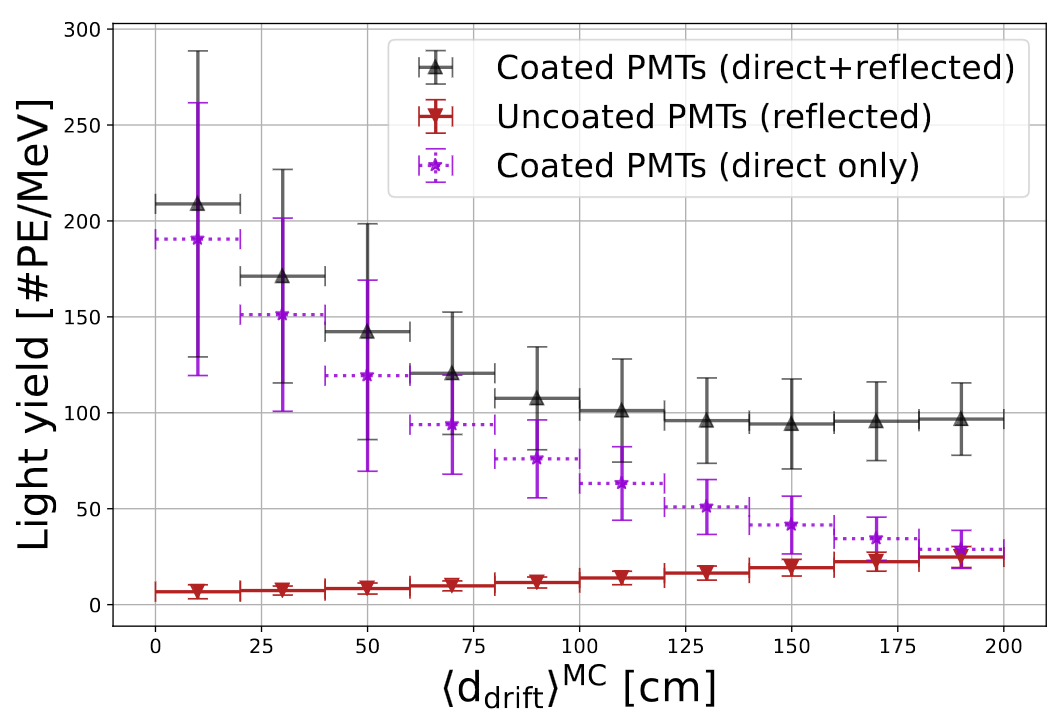
\includegraphics[width=0.55\textwidth]{light_yield_Diego}
\caption[light_yield_Diego]{
Expected light yield in SBND as a function of the mean drift distance collected by different types of PMTs.
The error bars show uncertainty due to geometrical effects of the detector.
Fig. from \cite{light_yield_Diego}.
}
\label{fig:light_yield_Diego}
\end{figure}


\section{Detection of Charge and Light}

\label{sec3:detection}

\subsection{Wire Readouts}

%TODO: add figures of signal shaping

Once arrive at the anode, the ionisation electrons induce signals on the readouts, which are typically made of three wire planes separated by a few mm as depicted in Fig. \ref{fig:LARTPC}.
A bias voltage is applied to each individual wire plane, allowing for electron transparency across the three planes.
As shown in Fig. \ref{fig:wire_current}, the drifted electrons induce bipolar signals on the two innermost planes as they pass through them; these planes are often referred to as the induction planes. 
The electrons are then collected on the outermost plane, producing a unipolar signal, and hence, this plane is commonly known as the collection plane.
The three planes are oriented 60$^{\circ}$ apart, minimising the impact of a particle travelling parallel to a wire plane.
While three-dimensional spatial reconstruction of a track requires a minimum of at least two wire planes, many modern LArTPC experiments use all three planes \cite{argoneut, icarus_det, ubooneDet, sbnd_det, protodune, dunefd_det}.
\begin{figure}[htp] 
\centering    
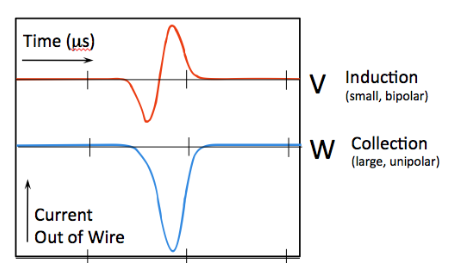
\includegraphics[width=0.57\textwidth]{wire_current}
\caption[wire_current]{
Current signals on the induction and collection wire plane, induced by a point-like charge deposition.
Fig. from \cite{argoneut}.
\hfill
\break
}
\label{fig:wire_current}
\end{figure}

The signals induced or collected on the wire planes are then shaped, amplified, and digitized by cold electronics before acquisition. 
The amount of charge collected is correlated with the energy deposited in the detector, accounting for additional corrections due to recombination and electron propagation effects as discussed in Sec. \ref{sec:recomb} and Sec. \ref{sec:edrift}. 
Finally, the spatial and calorimetry information allows for PID to be performed.


\subsection{Photomultiplier Tubes and X-ARAPUCA}

%Readout detection
Scintillation photons are detected by the Photon Detection System (PDS) located behind the wire planes, as depicted in Fig. \ref{fig:LARTPC}. 
The primary detection technology in the PDS is Photomultiplier Tubes (PMTs), which have a Quantum Efficiency (QE) of up to 30\% \cite{pmt_qe}.
However, PMTs are typically large and require sufficient volume inside the detector for installation. 
Current and future experiments are increasingly adopting Silicon Photomultipliers (SiPMs) due to their advantageous smaller size, lower power consumption, excellent signal-to-noise ratio, and a high QE of up to 40\% \cite{sipm_qe}.
The X-ARAPUCA device is a novel light collection technology utilising SiPMs, currently under development by Unicamp \cite{xarapuca} and being tested inside the SBND detector.
As shown in Fig. \ref{fig:xarapuca}, it is a light guide designed to trap light through a combination of a wavelength shifter and dichroic filters.
The dichroic filter is transparent to a narrow range of wavelengths and reflective otherwise, allowing only photons of specific wavelengths to pass through the filter and preventing their escape.
The photons are internally reflected in the trap until they are detected by the SiPMs.

\begin{figure}[htbp] 
\centering    
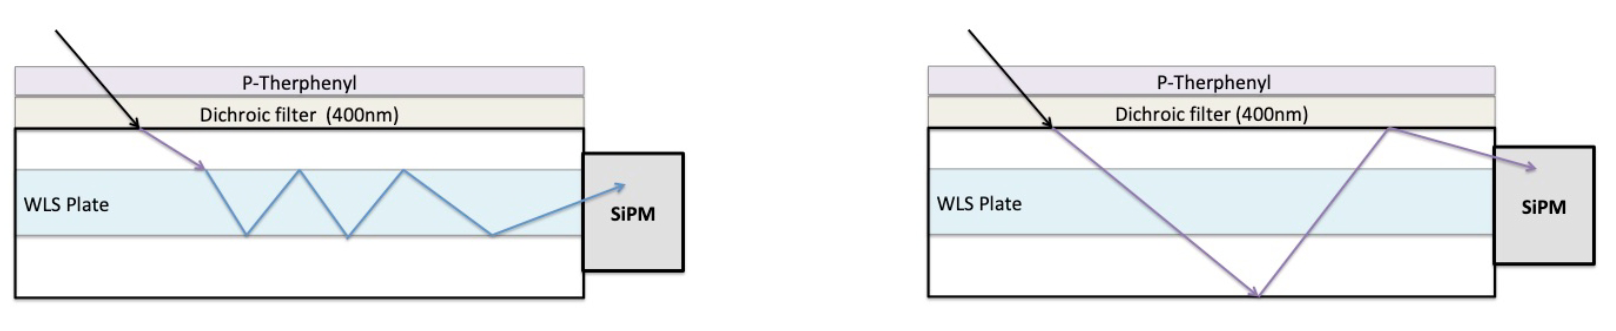
\includegraphics[width=1.0\textwidth]{xarapuca}
\caption[xarapuca]{
Diagram showing the operation principle of a X-ARAPUCA. 
The P-Therphenyl layer shifts 128 nm wavelength photons to 350 nm, allowing them to pass through the dichroic filter with a cut-off at 400 nm.
The 350 nm photons are trapped inside the reflective cavity until detected by SiPM (right).
The wavelength shifter plate converts the photons to 430 nm, trapping them by total internal reflection (left).
Fig. from \cite{xarapuca}.
\hfill
\break
}
\label{fig:xarapuca}
\end{figure}

As discussed in Sec. \ref{sec:wls}, both PMTs and X-ARAPUCAs are coated with TPB for wavelength shifting.
The re-emitted light direction is isotropic, causing coated optical detectors to suffer a 50\% reduction in efficiency due to photons emitting away from the detection surface.
TPB can also impact the detection time, as the emission of visible photons is not instantaneous.
Multiple time components of re-emitted photons from TPB have been observed, with the majority of photons re-emitted within nanoseconds and a subset re-emitted as long as a few microseconds \cite{tpb_time}.

Finally, the waveforms of the photons are digitized and acquired using a very high sampling frequency readout, ranging between 1-2 ns \cite{sbnd_det}.
This high sampling frequency gives the scintillation light signal much better timing resolution compared to the charge signal.
As a result, it provides the most precise interaction timing information available in the detector, which is particularly useful for triggering and Heavy Neutral Lepton analysis (See Chapter \ref{}).

%********************************** %First Section  **************************************
\section{Concluding Remarks}

Since the original proposal in 1977, LArTPCs have proven their potential as high precision neutrino detectors.
The understanding of particle interactions and their propagation within the detector, along with the detector's response to these particles, has significantly improved over time. 
Technological advancements in detection and readout now enable the scaling of LArTPCs from volumes of only several tons to even tens of kilotons, making them suitable for high multiplicity environments.
The next generation of LArTPCs aims to advance the field of neutrino physics, as outlined in the physics program of the SBND detector, which will be discussed in the following chapter.
